\documentclass{article}
\usepackage[left=2cm,right=2cm,top=2cm,bottom=2cm]{geometry}
\usepackage[utf8]{inputenc}
\usepackage[german]{babel}
\usepackage{amsmath}
\usepackage{dsfont}
\usepackage[export]{adjustbox}
\usepackage{amsthm}
\usepackage{color}
\usepackage{amsfonts}
\usepackage{amssymb}
\usepackage{wasysym}
\usepackage{makeidx}
\usepackage{graphicx}
\usepackage[colorlinks=true,urlcolor=blue,linkcolor=blue]{hyperref}
\usepackage{ziffer}
\usepackage{minted}
\usepackage{xcolor}
\usepackage{framed}
\usepackage{mdframed}
\usepackage{subfiles}
\usemintedstyle{emacs}

\definecolor{purp}{HTML}{9A72AC}
\definecolor{re}{HTML}{FC6255}
\definecolor{gre}{HTML}{83C167}
\definecolor{blu}{HTML}{58C4DD}
\definecolor{shadecolor}{rgb}{0.85,0.85,0.85}
\definecolor{bg}{rgb}{0.95,0.95,0.95}
\setlength{\parindent}{0em} 

\BeforeBeginEnvironment{minted}{\begin{mdframed}[linewidth =2 ,backgroundcolor=bg , linecolor=black, linewidth=0.5]}
\AfterEndEnvironment{minted}{\end{mdframed}}

\newtheorem{defi}{Definition}
\BeforeBeginEnvironment{defi}{\begin{mdframed}[linewidth =2 ,backgroundcolor=bg , linecolor=black, linewidth=0.5]}
\AfterEndEnvironment{defi}{\end{mdframed}}

\newcommand{\bsp}{\textbf{Beispiel}:}
%\newcommand{\task}{\textbf{Aufgabe}:}

\newcommand{\bol}[1]{\textbf{#1}}
\newcommand{\q}[1]{\glqq #1\grqq}
\newcommand{\DODO}[1]{\textbf{\textcolor{red}{DODO:}} #1 \\ \begin{center}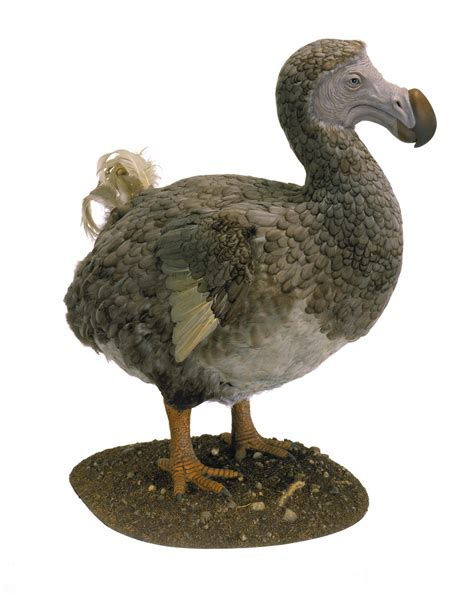
\includegraphics[scale=0.2]{../../media/dodo.jpg} \end{center}}

\newenvironment{task}[1]{
    \begin{shaded*}
    \textbf{Aufgabe #1}:
}{
    \end{shaded*}
}

\begin{document}

Für die Länge der Warteschlange soll der Endknoten nicht zählen, d.h. es wird nur die Anzahl der Datenknoten benötigt. Die Frage nach der Länge wird also bis zum Endknoten durchgereicht, dieser antwortet mit 0, alle anderen zählen zum Ergebnis ihres Vorgängers eins dazu und geben weiter zurück. \\
\bsp Der letzte Datenknoten erhält vom Endknoten die $0$, addiert $1$ und gibt an den vorletzten $1$ zurück. Dieser addiert wiederum $1$ und gibt $2$ weiter zurück, usw.
\begin{minted}{Java}
    //class MyListComp 
    public int length() {
        return root.length();
    }    

    //class Node 
    public abstract int length();

    //class DataNode 
    @Override
    public int length() {
        return next.length() + 1;
    }

    //class EndNode 
    @Override
    public int length() {
        return 0;
    }
\end{minted}
Um ein Datenelement an einer bestimnmten Position zu finden müssen wir wieder auf das Konzept des Zählers, der durchgereicht wird, zurückgreifen. Die Abfrage, ob die Liste kürzer als die gesuchte Position ist können wir umgehen, indem wir den Endknoten null zurückgeben lassen, sollte er erreicht werden. Wie in früheren Beispielen soll in dieser Implementierung außerdem das Zählen bei $1$ beginnen, d.h. die Wurzel ist der erste und nicht der \q{Nullte} in der Reihe.
\begin{minted}{Java}
    //class MyListComp
    public DataElement itemAtPosition(int position){
        int counter = 1;
        DataElement found = root.itemAtPosition(position, counter);
        return found;
    }

    //class Node 
    public abstract itemAtPosition(int position, int counter);

    //class DataNode 
    @Override
    public DataElement itemAtPosition(int position, int counter) {
        if(counter == position){
            return this.getData();
        } else {
            return next.itemAtPosition(position, counter + 1);
        }
    }

    //class EndNode 
    @Override
    public DataElement itemAtPosition(int position, int counter) {
        return null;
    }
\end{minted}
Die Methode, die in der Schlange sucht folgt der exakt selben Logik, nur gibt hier der Endknoten die (willkürlich) festgelegte -1 statt null zurück:
\begin{minted}{Java}
    //class MyListComp
    public int searchItemInQueue(DataElement data) {
        int counter = 1;
        int position = root.searchItemInQueue(data,counter);
        return position;
    }

    //class Node 
    public abstract int searchItemInQueue(DataElement data, int counter);

    //class DataNode 
    @Override
    public int searchItemInQueue(DataElement data, int counter) {
        if(this.getData().equals(data)){
            return counter;
        } else {
            return next.searchItemInQueue(data, counter +1);
        }
    }

    //class EndNode 
    @Override
    public int searchItemInQueue(DataElement data, int counter) {
        return -1;
    }
\end{minted}
Wie immer kann für die enthält()-Methode ein eigener rekursiver Durchlauf verwendet werden, oder es wird auf die Methode aus der vorherigen Aufgabe zurückgegriffen, diesmal in der kürzeren Variante: 
\begin{minted}{Java}
    //class MyListComp 
    public boolean contains(DataElement data) {
        if(this.searchItemInQueue(data) != -1) {
            return true;
        } else {
            return false;
        }
    }
\end{minted}
Die Methode, die an einer beliebigen Stelle entfernt, kann auf die vorneEntfernen()-Methode zurückgreifen, falls die spezifizierte Position der ersten entspricht. Andernfalls wird wieder ein Zähler benötigt, die Struktur sieht völlig analog zu früheren Varianten aus (der Endknoten wird wieder null zurückgeben!): 
\begin{minted}{Java}
    //class MyListComp 
    public DataElement removeAtPosition(int position) {
        if(position <= 0) {
            return null;
        }
        if(position == 1) {
            return this.pop();
        } else {
            int counter = 1;
            return root.removeAtPosition(position, counter);
        }
    }

    //class Node 
    public abstract DataElement removeAtPosition(int position, int counter);

    //class DataNode 
    @Override
    public DataElement removeAtPosition(int position, int counter){
        if(counter == position - 1){
            DataElement toReturn = next.getData();
            next = next.getNext();
            return toReturn; 
        } else {
            return next.removeAtPosition(position, counter + 1);
        }
    }

    //class EndNode 
    @Override
    public DataElement removeAt(int position, int counter){
        return null;
    }
\end{minted}
In der Liste wird nur auf der Wurzel das Entfernen auf der Wurzel gestartet. Da die Wurzel in jedem Fall mindestens ein Endknoten ist, entfällt wiederum eine Prüfung, ob die Liste leer ist. Ein Endknoten gibt nur sich selbst zurück und es entsteht kein Schaden. Durch die Implementierung auf diese Weise ist allerdings keine Bestätigung der Ausführung möglich, da für das \q{elegante} Durchreichen eine Rückgabe des Knotens notwendig ist. \\
Im Datenknoten wird überprüft, ob das übergebene Element identisch mit dem Inhalt dieses Knotens ist (dazu wird wieder die vergleichsMethode des Datenelements genutzt!). Falls dies der Fall ist, wird der Nachfolger des Knotens zurückgegeben. Dadurch erhält sein Vorgänger eine Referenz auf den Nachfolger und der Knoten mit den gesuchten Daten ist entfernt. 
\begin{minted}{Java}
    //class MyListComp 
    public void removeElement(DataElement toRemove) {
        root = root.removeElement(toRemove);
    }

    //class Node 
    public abstract Node removeElement(DataElement toRemove);

    //class DataNode 
    public Node removeElement(DataElement toRemove) {
        if(toRemove.getData().equals(data.getData())) {
            return next;
        } else {
            next = next.removeElement(toRemove);
        }
        return this;
    }

    //class EndNode 
    public Node removeElement(DataElement toRemove) {
        return this;
    }
\end{minted}

\end{document}